\section{Bedienung}\label{text:Entwicklung-des-Stellwerks:Bedienung}

Der Einfachheit halber wurde auf die Entwicklung einer grafischen Benutzeroberfläche in Anlehnung an ein \ac{ESTW}, verzichtet. Stattdessen wurde eine Kommandozeilenapplikation entwickelt, deren Bedienung an die der ersten \ac{ESTW}s angelehnt ist. \autoref{abb:Entwicklung-des-Stellwerks:Bedienung} zeigt die Oberfläche beispielhaft.

\begin{figure}[H]
    \centering
    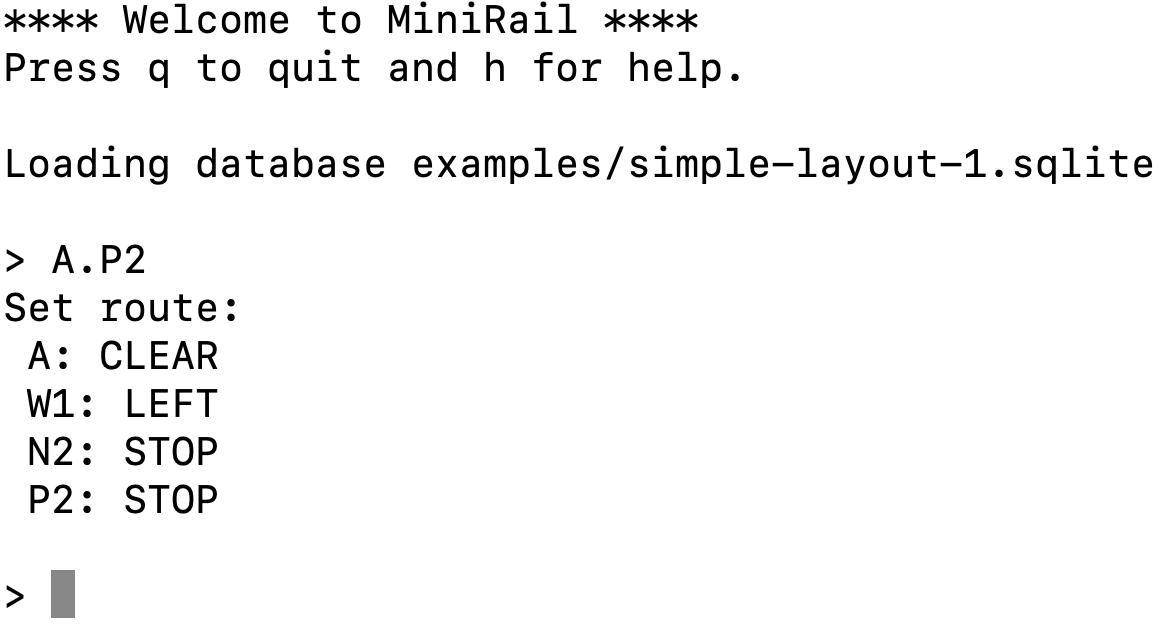
\includegraphics[width=.8\textwidth]{Assets/Images/5-Entwicklung-des-Stellwerks/Bedienung.png}
    \caption{Bedienoberfläche des Stellwerks}\label{abb:Entwicklung-des-Stellwerks:Bedienung}
\end{figure}

Die Topologie der Gleisanlage ist in einer SQLite-Datenbank gespeichert, welche beim Programmstart übergeben wird. Über einen \textit{Bedienstring} wird das Stellwerk gesteuert. Die Syntax ist hier immer \texttt{<start>.<ziel>} und hat das Stellen einer Zugfahrstraße von \texttt{start} nach \texttt{ziel} zur Folge.

Da die einzelnen Komponenten nicht miteinander kommunizieren können, handelt sich die Ausgabe um eine Simulation. Signale und Weichen werden also nicht wirklich gestellt.
